\documentclass[lettersize,journal]{IEEEtran}
\usepackage{hyperref}
\usepackage{amsmath,amsfonts}
\usepackage{algorithmic}
\usepackage{algorithm}
\usepackage{array}
\usepackage[caption=false,font=normalsize,labelfont=sf,textfont=sf]{subfig}
\usepackage{textcomp}
\usepackage{stfloats}
\usepackage{url}
\usepackage{verbatim}
\usepackage{graphicx}
\usepackage[font=footnotesize,justification=centering]{caption}
\usepackage{cite}
\hyphenation{op-tical net-works semi-conduc-tor IEEE-Xplore}
% updated with editorial comments 8/9/2021
\usepackage{subfig}
\usepackage{amssymb}





\begin{document}





\title{Post Delivery Robot Simulation using Templar Difference}

\author{Mohamad Ali Saber \\ \href{mailto:malisaber@yahoo.com}{malisaber@yahoo.com}}
\maketitle

\begin{abstract}
In this computer assignment, we dive into find the optimal policy for a Post Delivery Robot using Monte Carlo (MC) algorithm. The RL agent is a car in a 5 by 5 grid world environment trying to pick up the postal package in one of the pre-defined location. The agent interacts with the environment to find the best action in each state. It can move in the four main direction that are North, East, South, and West and also pick up a package. It receives a reward based on the action that it takes. The reward function generates in a way that guide the agent to find the shortest path to the postal box and punished it whenever it picks the wrong box.\par

The objective of this computer assignment is to develop and compare On-Policy and Off-Policy Templar Difference (TD) control algorithm for policy improvement. At first, the agent tries to learn the optimum policy by looking one step ahead which is TD(0). Then using 4 steps ahead which is TD(4) and compare their results.\par

To visualize the results, the action map and state value of each different location of the postal package for two learning methods have been plotted. And lastly, to have a comparison between these two methods, the average return of each algorithm per episode have been plotted. The results show that both SARSA and Q-learning in both 1-step and 4-step were able to find a near optimum policy. However, in term of rewards, the 4-step SARSA performs the best.
\end{abstract}

\begin{IEEEkeywords}
Reinforcement Learning, Templar Difference, SARSA, Q-Learning, Policy.
\end{IEEEkeywords}




%%%%%%%%%%%%%%%%%%%%%%%%%%%%%%%%%%%%%%%%%%%%%%%%%%%%%%%%%%%%%%%%%%%%%%%%%%%%%%%%%%
%                   INTERODUCTION
%%%%%%%%%%%%%%%%%%%%%%%%%%%%%%%%%%%%%%%%%%%%%%%%%%%%%%%%%%%%%%%%%%%%%%%%%%%%%%%%%%
\section{Introduction}
\IEEEPARstart{K}{nowledge} of environment helps the humankind to propose a complete model of that environment and also have a perfect and complete control over that environment, but in some cases, the under study environment become too complex to find the mathematical model of that environment or calculating the mathematical model of it becomes too computationally intensive that proposing the model is not a cost-efficient task. Basic Reinforcement Learning algorithms use the complete model of environment to find the best control over that, but those algorithms fail when there is no accurate or complete model available. in this case, scientists propose a new types of RL algorithms that learns from the previous experience of an agent within that environment to find the best action in each states of the environment. Templar Difference algorithms such as the SARSA and the Q-Learning are model-free and experiment-based learning algorithms that learns the near best and best action from directly interacting with the environment.\par

The environment is a 5×5 discrete grid representing the operational area of a delivery robot. The robot can move north, south, east, or west, or attempt to pick up a package using a fifth action. Any attempts to exit the world is useless and brings the robot to its last location. At the start of each episode, the robot's position is randomized, and the package is placed at one of four fixed places. The robot's actions are deterministic, but any attempt to move outside the grid results in a penalty. Also, there are some walls within the grid world that limits the movement of the robot, by punishing the robot every times that it hits any of these walls, the robot learns to move around them when any wall is in its path.\par

The episode ends either when the package is picked up successfully or after 25 steps. The reward structure encourages efficient and accurate behavior, with +20 for a correct pickup, –10 for illegal moves (i.e. exiting the world and hitting the walls) or incorrect pickups, and –1 for each time step to discourage delays. This environment provides a clear, structured setting for training and evaluating Monte Carlo control algorithms. \par




The following of this report is organized az:
\begin{itemize}
    \item Section II: methodology of the solution
    \item Section III: a brief explanation of the implemented code
    \item Section IV: simulation results
    \item Section V: Conclusion
\end{itemize}
\vspace{0.3cm}


%%%%%%%%%%%%%%%%%%%%%%%%%%%%%%%%%%%%%%%%%%%%%%%%%%%%%%%%%%%%%%%%%%%%%%%%%%%%%%%%%%
%                  Methodology
%%%%%%%%%%%%%%%%%%%%%%%%%%%%%%%%%%%%%%%%%%%%%%%%%%%%%%%%%%%%%%%%%%%%%%%%%%%%%%%%%%
\section{Methodology}
In this section, a brief explanation of the model will be presented. This section contains four subsections to cover the state model, action model, reward model, and Environment model of the RL agent.\par

\subsection{State Model}
The state model should covers all the possible configurations of the car and the postal package position. Since the world is a 5 by 5 discrete environment it can have 25 distinguishable positions and therefore 25 different positions to represent the coordinates of the robot. Also there is 4 different possible locations for the package that has a direct effect on the agent behavior and should be concluded as the state of the environment. Therefore, the state vector defined as below with total 100 possible different states.

\begin{equation}
S = [x, y, p]
\end{equation}

where x and y denote as the x and y coordinate of the car, respectively, and p represents the number of package.

\subsection{Action Model}
To have the full access to each position of the map, the robot should be capable of moving in all 4 main directions as North, East, South, and West. The fifth action defined as picking up the package. Therefore, the action space defined as bellow:

\begin{equation}
A = [N, E, S, W, P]
\end{equation}


\subsection{Reward Model}
The agent required to find the shortest path to the package, avoid hitting to the wall, staying within the world, and pick up the right package. To guide the agent to achieve these goals, the reward function describes as following, a -1 reward to each action within the world, -10 points when the agent tries to leave the world, hitting the inner walls, and picking the wrong package, and last, a +20 when it picks the right package.


\subsection{Environment Model}
Environment modeled through its 4-argument transition probability function. Therefore environment uses its transition probability to find the next state and reward based on present state and taken action.


%%%%%%%%%%%%%%%%%%%%%%%%%%%%%%%%%%%%%%%%%%%%%%%%%%%%%%%%%%%%%%%%%%%%%%%%%%%%%%%%%%
%                 Implementation
%%%%%%%%%%%%%%%%%%%%%%%%%%%%%%%%%%%%%%%%%%%%%%%%%%%%%%%%%%%%%%%%%%%%%%%%%%%%%%%%%%
\section{Implementation}
In this section, three main implemented functions that are Environment class, On-Policy and Off-Policy, will be explained.



\subsection{Environment}
The Environment class has been developed, this class contains some physical information of the environment like position of the robot and package and dynamics of the environment, and other intellectual information like episode length etc. This class contains some fundamental function to generate and simulate the environment using the given policy, and also plot the results. Figure \ref{fig:env_class} shows some implemented function within the environment class and figure \ref{fig:env} shows a frame of simulation.


\begin{figure}
    \centering
    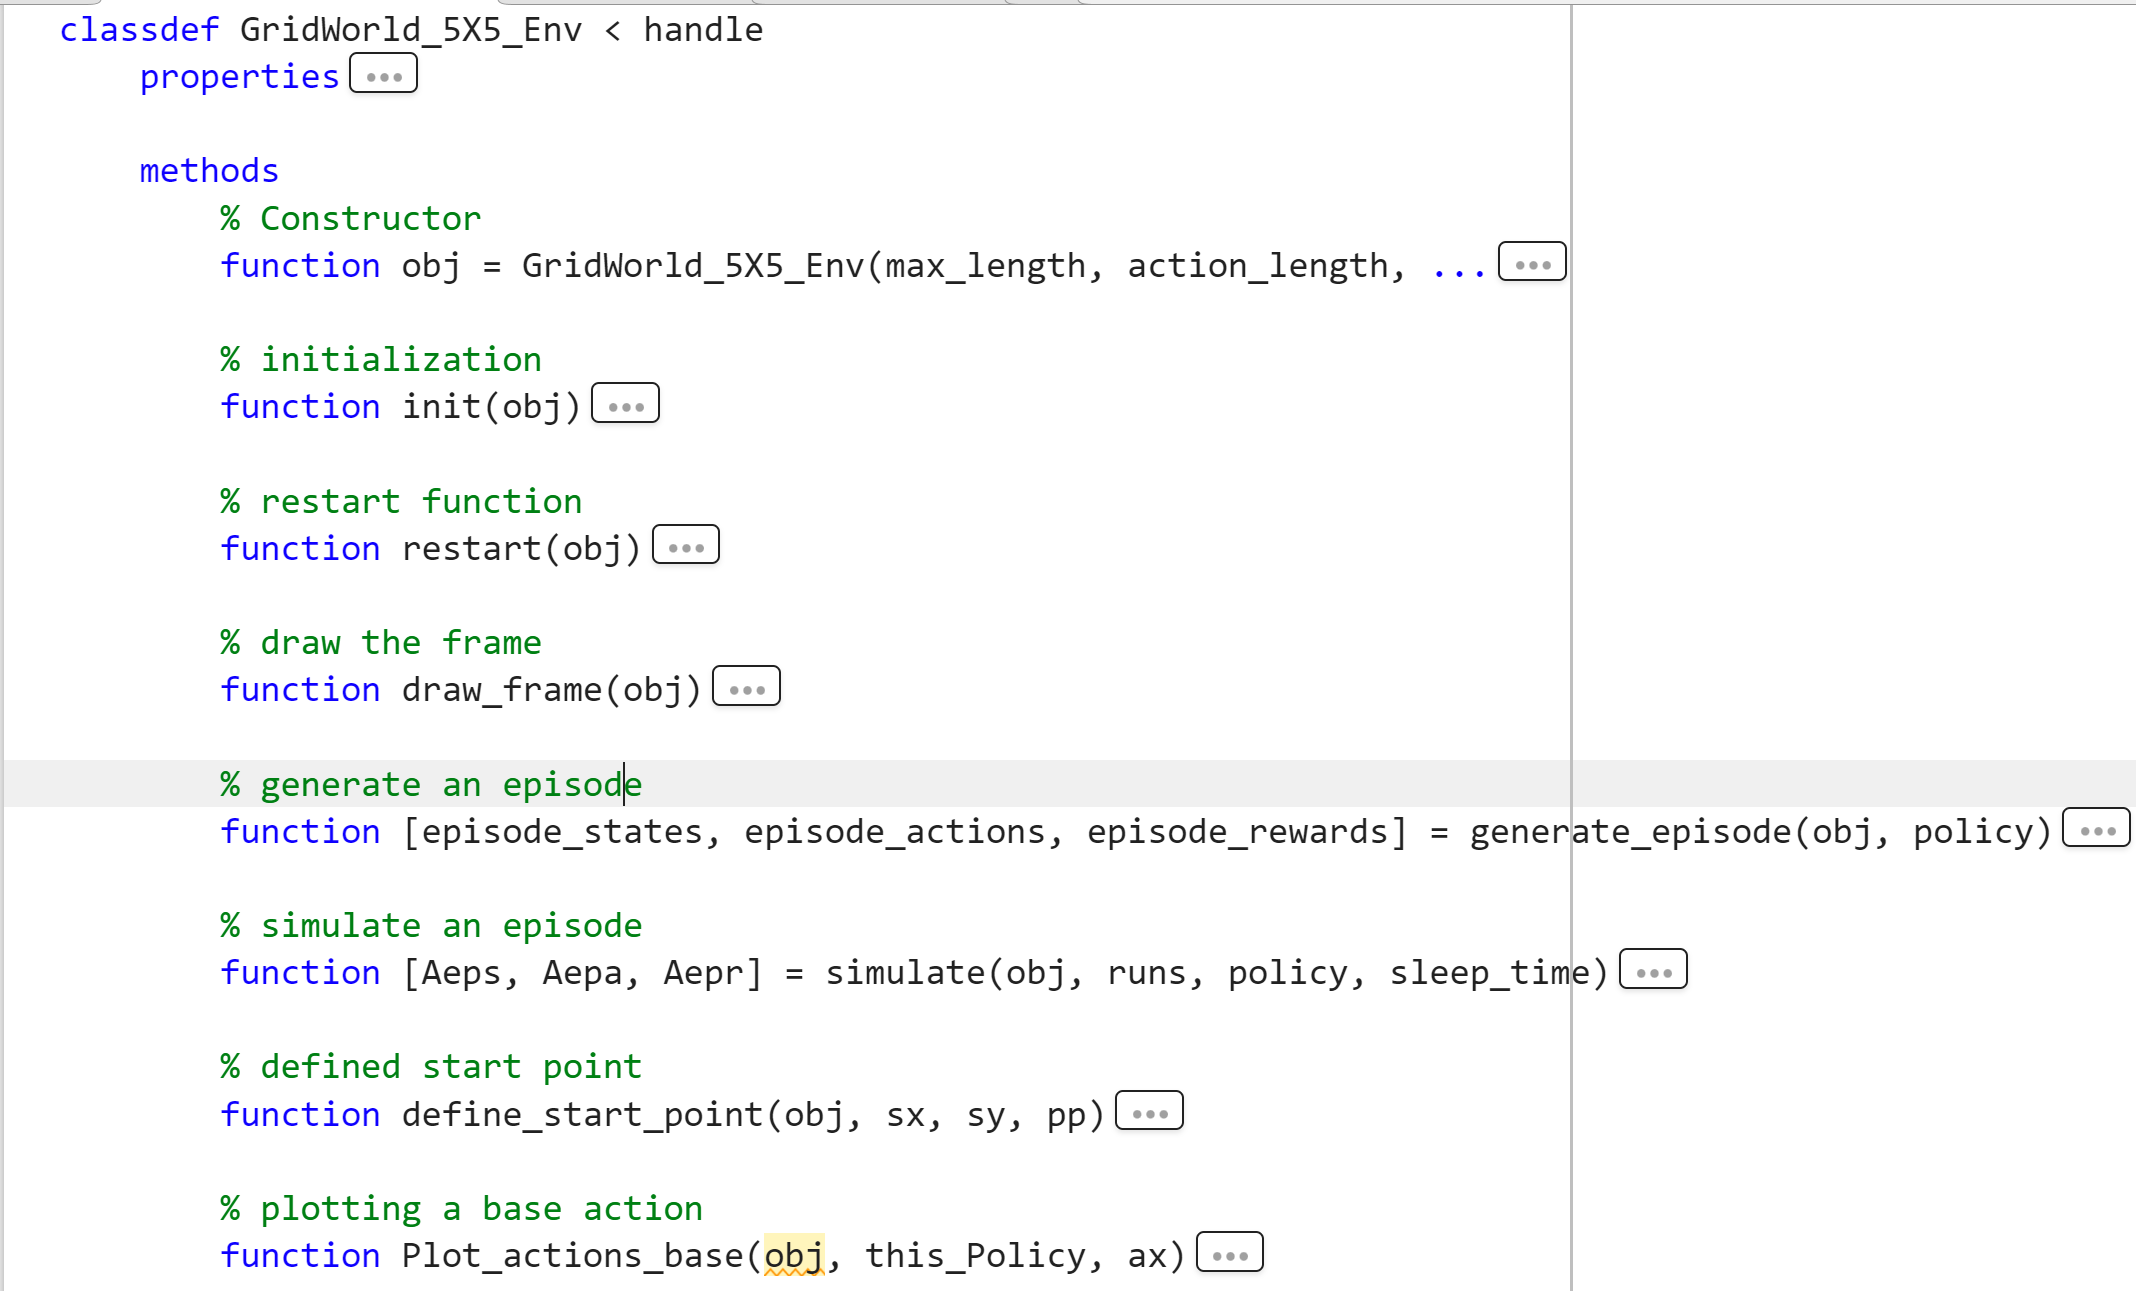
\includegraphics[width=1\linewidth]{pics/env_class.PNG}
    \caption{\centering some function of the environment class}
    \label{fig:env_class}
\end{figure}

\begin{figure}
    \centering
    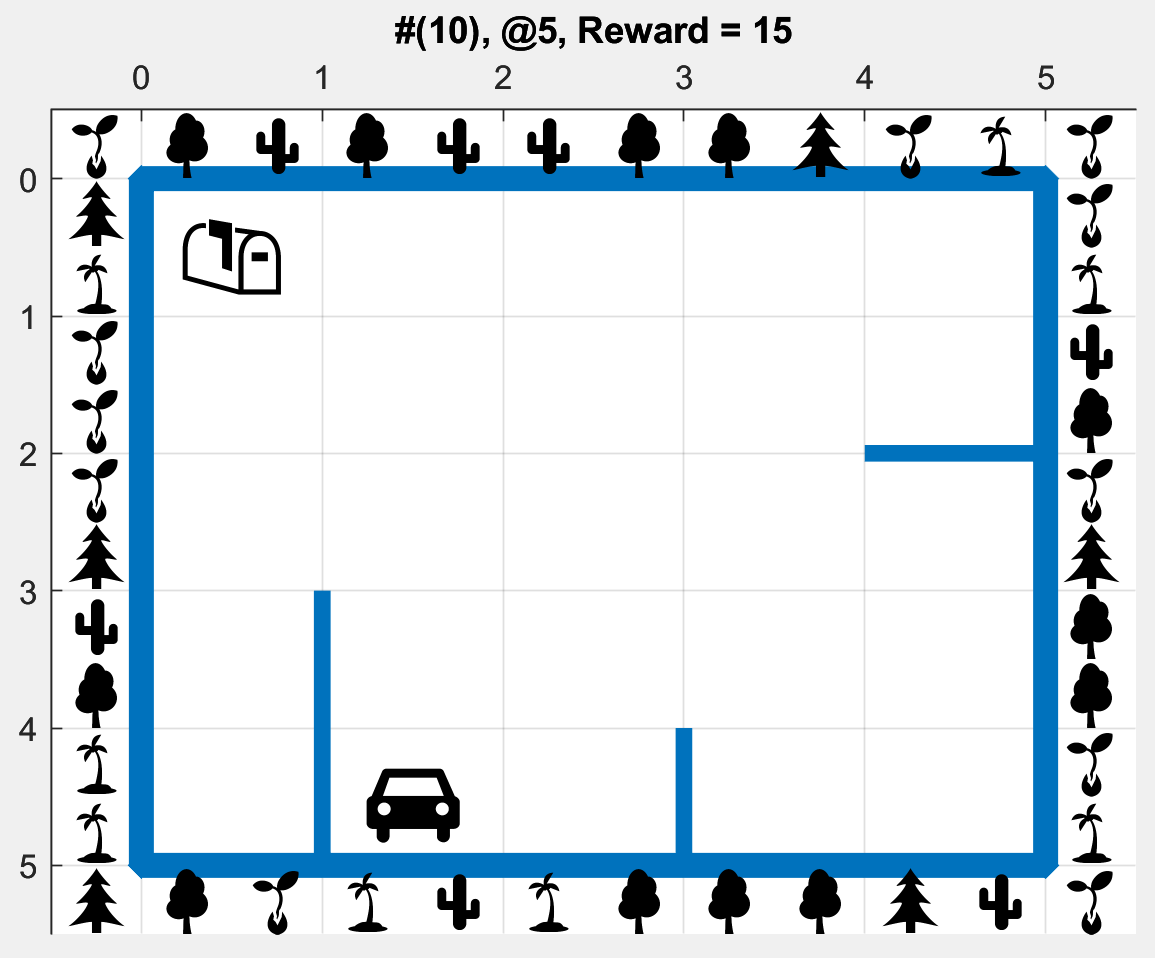
\includegraphics[width=1\linewidth]{pics/env.PNG}
    \caption{\centering a simulation frame}
    \label{fig:env}
\end{figure}



\subsection{One Step SAARS}
The 1 Step SAARS algorithm implemented under a function with the same name. Within the function, at each episode, the environment resets and the package and the robot respawn randomly. Then the environment generate an action using policy derived from calculated Q values and observe its reward and the next state. For each step of that episode, action-value of corresponded episode updates. This routine repeats for 100,000 times and then returns the generated policy and corresponded action-value matrix.



\subsection{One Step Q-Learning}
The 1-step Q-Learning algorithm declared in separate file, the overall structure of this function is the same as the SARSA function with minor difference in the updating of action-value matrix.


\subsection{Four Step SAARS and Q-Learning}
Implementation of 4-step TD algorithms are similar to 1-step TD implementations. The only difference is that in -step TD algorithms, the agent learn on four consecutive steps.

In the main script, at first, some variables have been initialized, then the dynamics of the environment has been generated and after that, an instantiation of the environment has been instanced. At the end, all four above mentioned implementation have been called. For each, its corresponded policy has been generated and the environment simulate the policy in 30 steps.


%%%%%%%%%%%%%%%%%%%%%%%%%%%%%%%%%%%%%%%%%%%%%%%%%%%%%%%%%%%%%%%%%%%%%%%%%%%%%%%%%%
%                  simulation results
%%%%%%%%%%%%%%%%%%%%%%%%%%%%%%%%%%%%%%%%%%%%%%%%%%%%%%%%%%%%%%%%%%%%%%%%%%%%%%%%%%
\section{simulation results}
All TD control algorithms learn on 100,000 episodes, with $\gamma$ of 1 and $\epsilon$ equal to 0.01. However, the 4-step Q-learning algorithm starts with $\epsilon$ equal to 1 and decay its value by 0.9 every 1000 episodes. predicted policies using 1-step SARSA, 1-step Q-Learning, 4-step SARSA, and 4-step Q-Learning are depicted in figures \ref{fig:sarsa_policy}, \ref{fig:QL_policy}, \ref{fig:n4_sarsa_policy}, and \ref{fig:n4_QL_policy}, respectively. As you can see, all four policies are near optimum and do not contain any irregularities. Furthermore, color map of all state values are shows in figures \ref{fig:sarsa_Vs}, \ref{fig:QL_Vs}, \ref{fig:n4_sarsa_Vs}, and \ref{fig:n4_QL_Vs}, respectively. Once more, all of four algorithm generates the same value functions which indicates that the implementation was correct. 


\begin{figure}
    \centering
    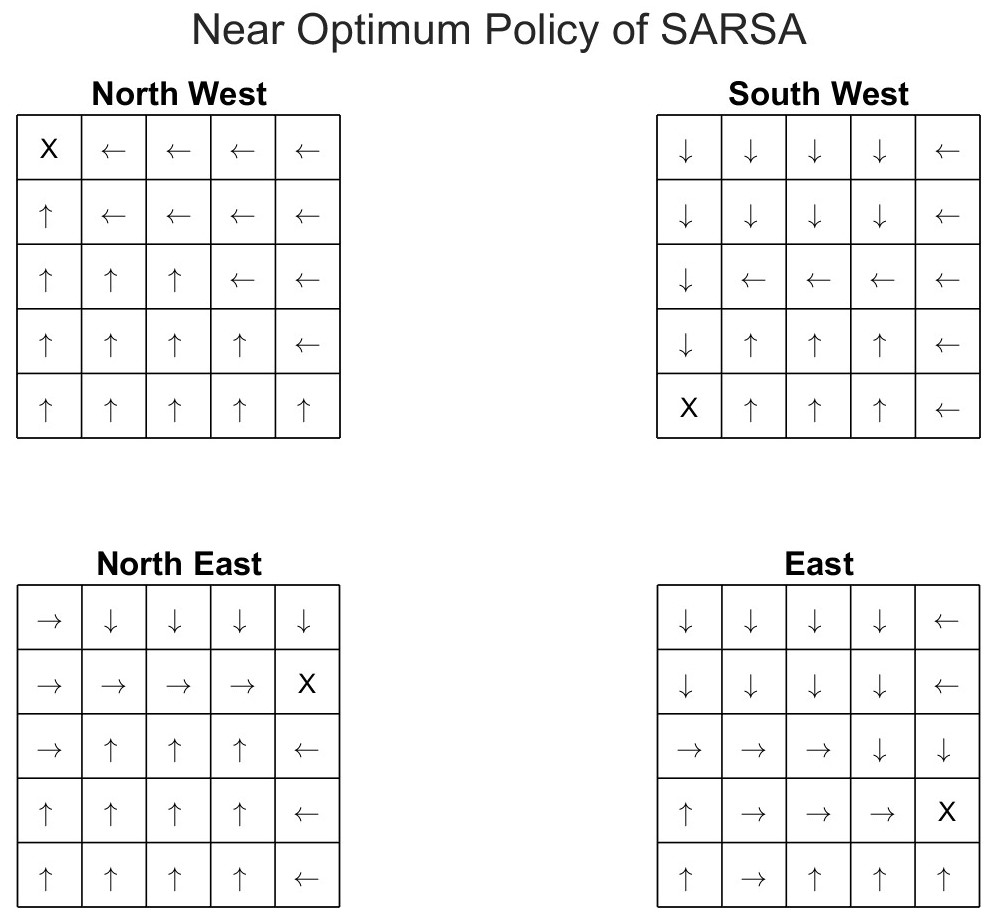
\includegraphics[width=1\linewidth]{pics/sarsa_policy.jpg}
    \caption{\centering Action Map of the 1-step SARSA predicted policy for different package positions}
    \label{fig:sarsa_policy}
\end{figure}

\begin{figure}
    \centering
    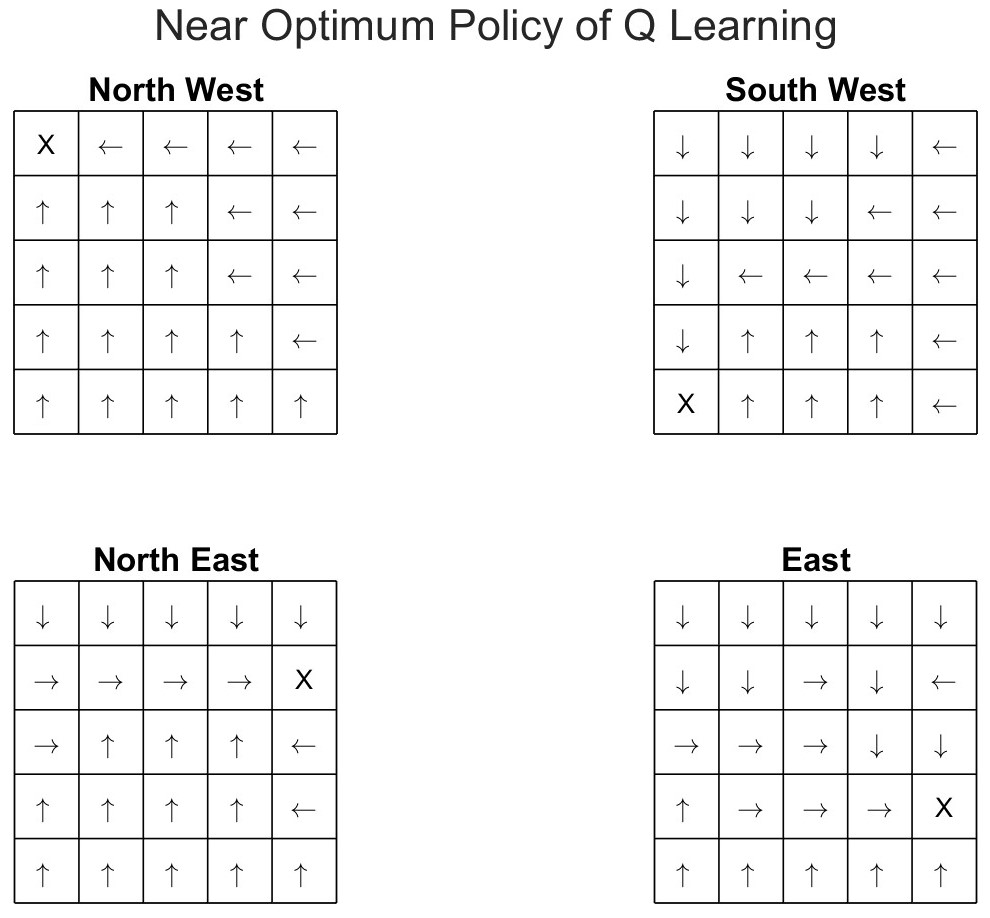
\includegraphics[width=1\linewidth]{pics/QL_policy.jpg}
    \caption{\centering Action Map of the 1-step Q-Learning predicted policy for different package positions}
    \label{fig:QL_policy}
\end{figure}


\begin{figure}
    \centering
    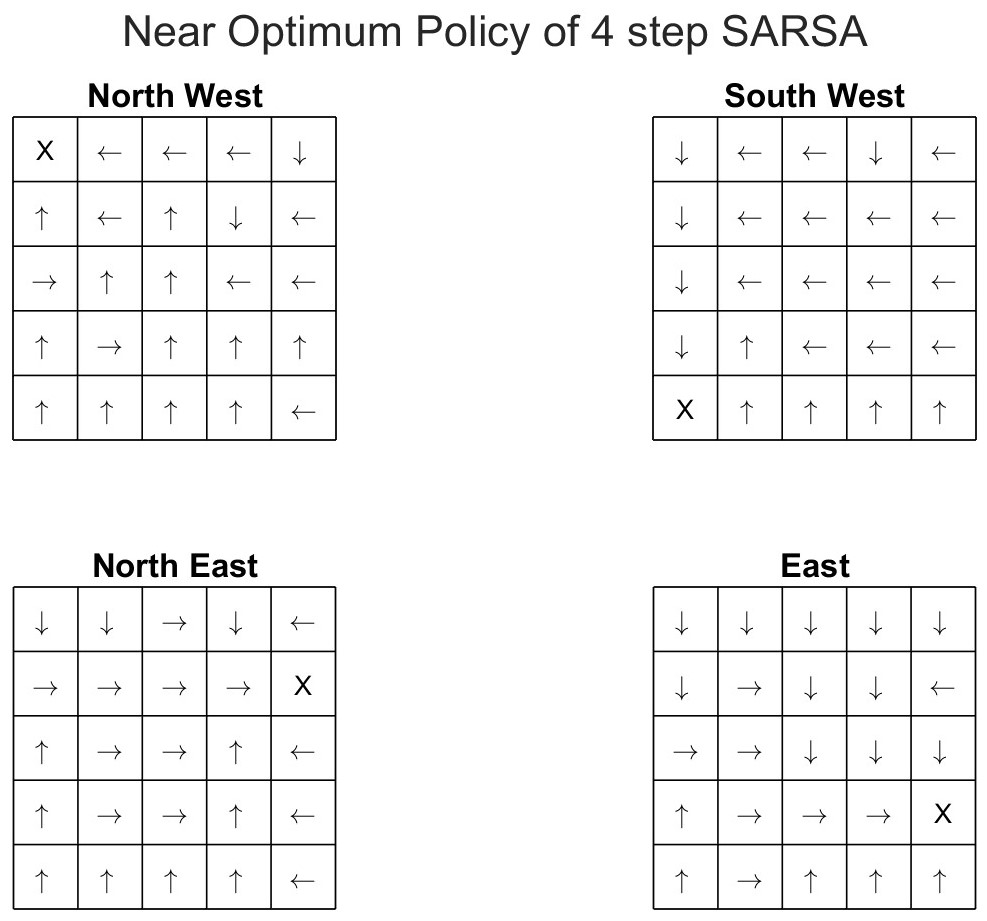
\includegraphics[width=1\linewidth]{pics/n4_sarsa_policy.jpg}
    \caption{\centering Action Map of the 4-step SARSA predicted policy for different package positions}
    \label{fig:n4_sarsa_policy}
\end{figure}

\begin{figure}
    \centering
    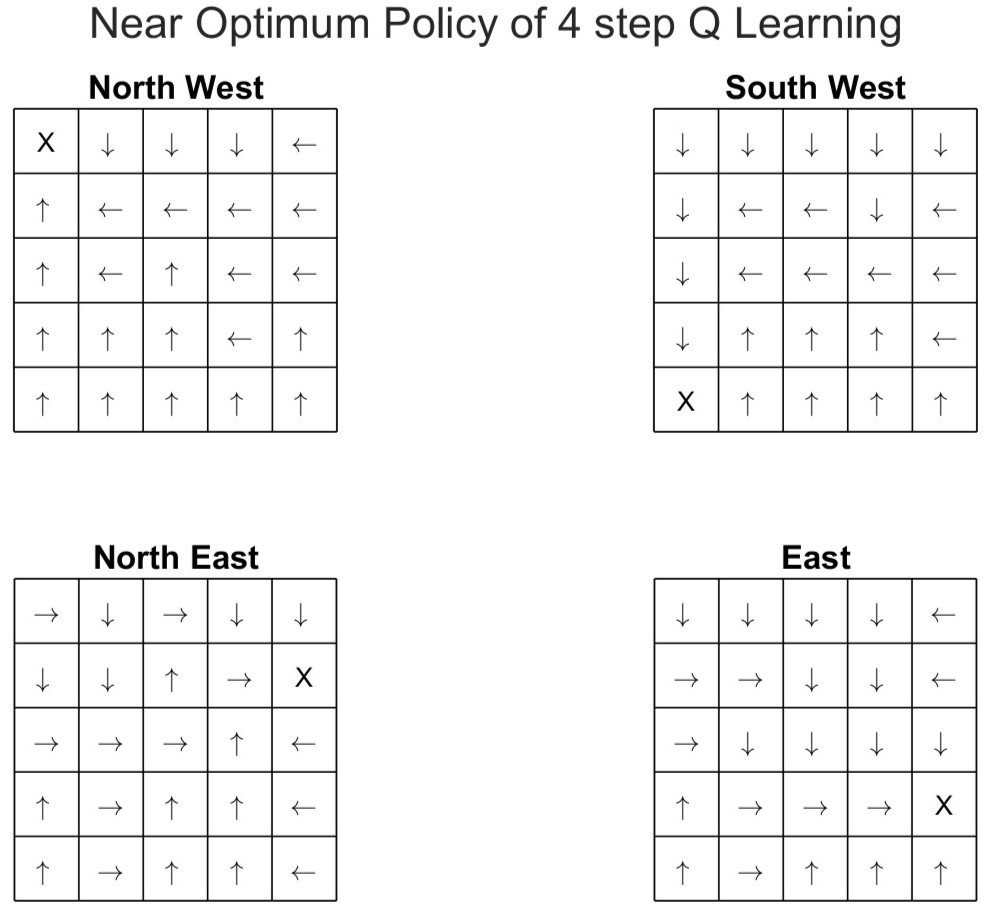
\includegraphics[width=1\linewidth]{pics/n4_QL_policy.jpg}
    \caption{\centering Action Map of the 4-step Q-Learning predicted policy for different package positions}
    \label{fig:n4_QL_policy}
\end{figure}


\begin{figure}
    \centering
    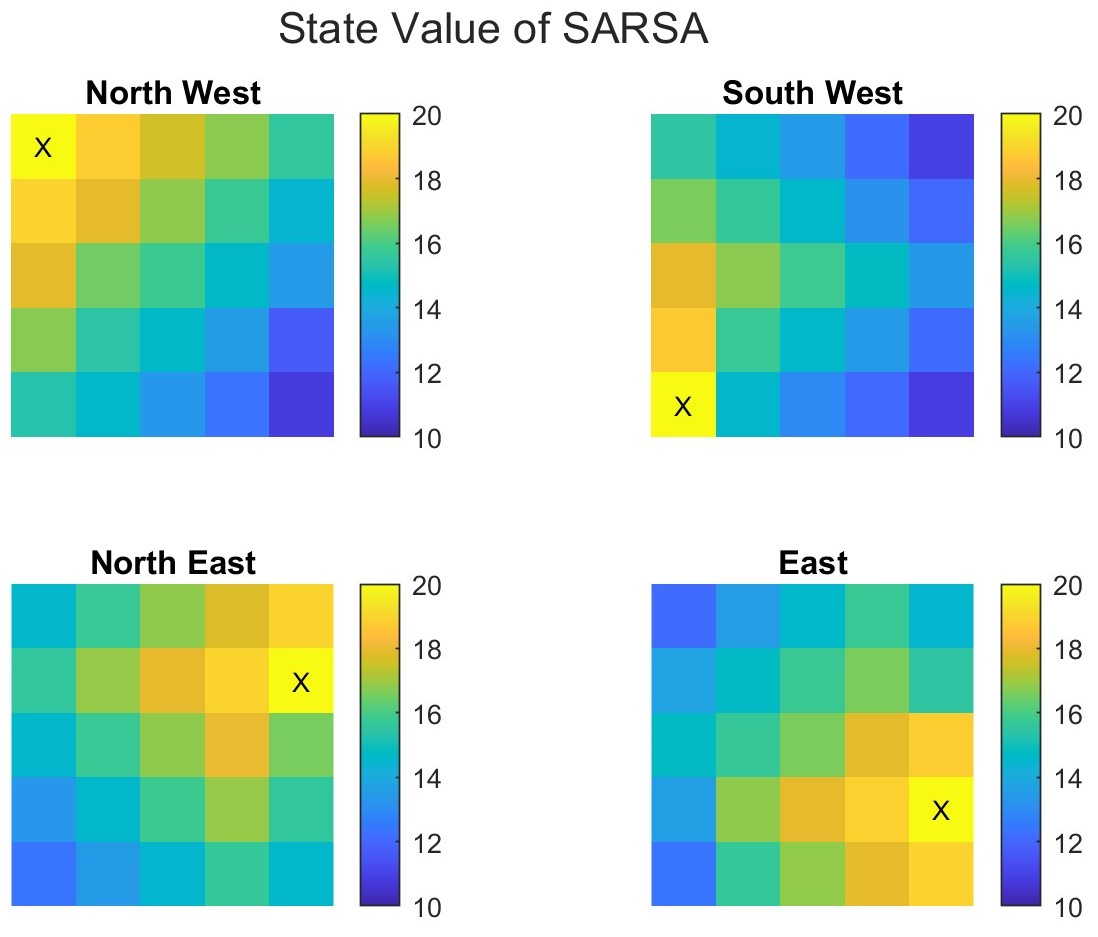
\includegraphics[width=1\linewidth]{pics/sarsa_Vs.jpg}
    \caption{\centering State Value of the 1-step SARSA method}
    \label{fig:sarsa_Vs}
\end{figure}

\begin{figure}
    \centering
    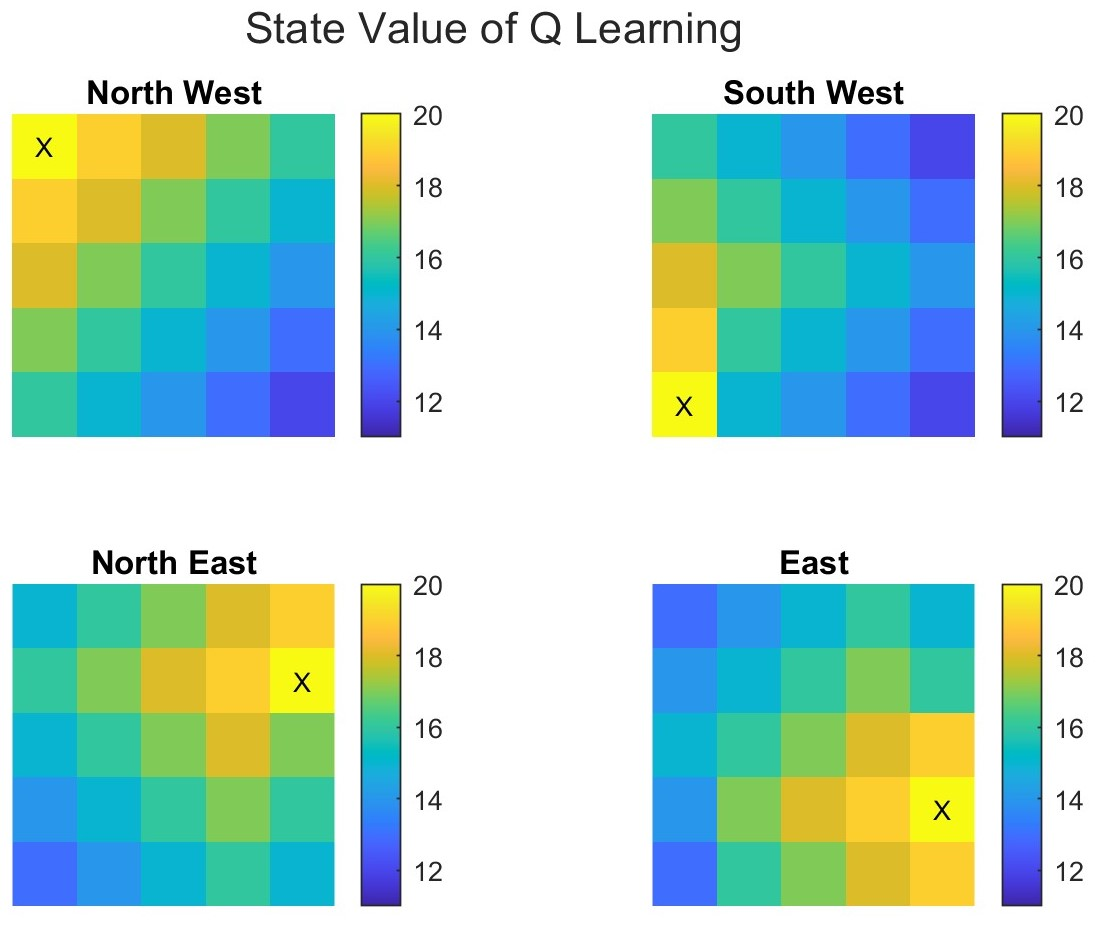
\includegraphics[width=1\linewidth]{pics/QL_Vs.jpg}
    \caption{\centering State Value of the 1-step Q-Learning method}
    \label{fig:QL_Vs}
\end{figure}


\begin{figure}
    \centering
    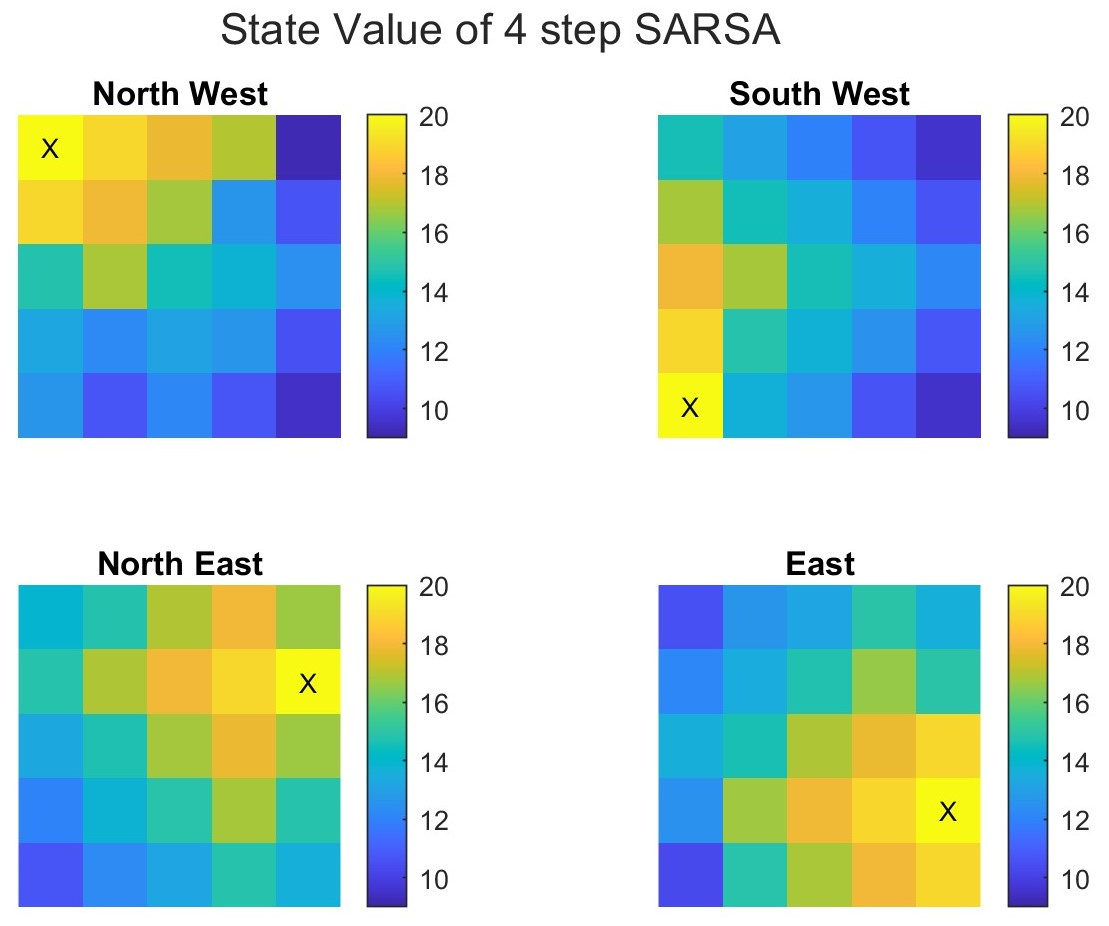
\includegraphics[width=1\linewidth]{pics/n4_sarsa_Vs.jpg}
    \caption{\centering State Value of the 4-step SARSA method}
    \label{fig:n4_sarsa_Vs}
\end{figure}

\begin{figure}
    \centering
    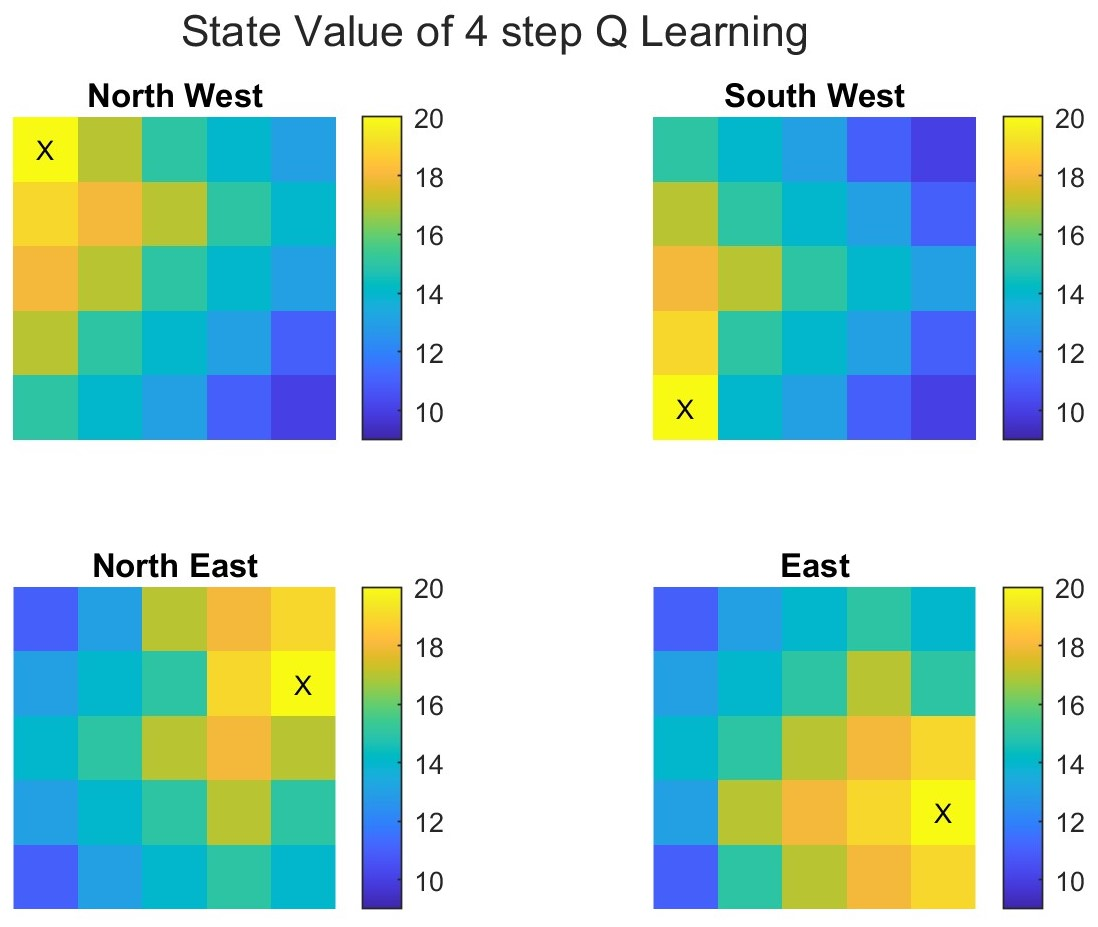
\includegraphics[width=1\linewidth]{pics/n4_QL_Vs.jpg}
    \caption{\centering State Value of the 4-step Q-Learning method}
    \label{fig:n4_QL_Vs}
\end{figure}

\begin{figure}
    \centering
    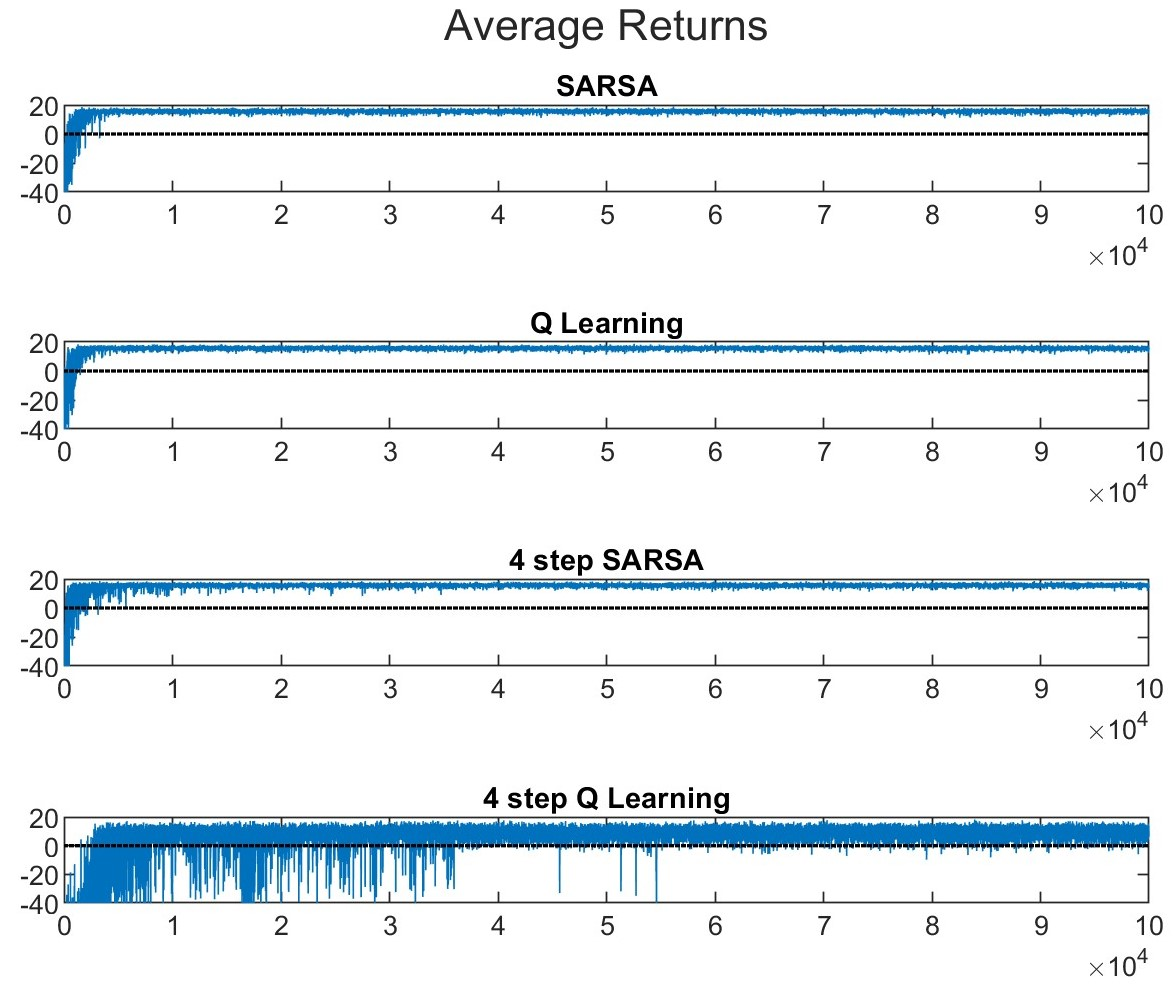
\includegraphics[width=1\linewidth]{pics/Comp.jpg}
    \caption{\centering Average rewards of different control method over all episodes}
    \label{fig:comp}
\end{figure}

Figure \ref{fig:comp} presents the average return per episode for all four Templar Difference control strategies. Each curve represents the agent’s learning performance over 100,000 episodes, providing insight into how quickly and effectively each method converges toward optimal behavior.

The first subplot shows the performance of the 1-step SARSA method using a constant $\epsilon$-greedy strategy. The return starts low—around –30 to –40 due to frequent illegal actions and inefficient paths in early exploration. Over time, the average return improves and eventually stabilizes, although it remains noisy and does not consistently reach the optimal return level. This indicates that the agent struggles to fully converge due to suboptimal updates caused by early exploratory actions.

The second subplot illustrates the 1-step Q-learning TD method. This approach starts low similar to the previous method, but quickly achieves near-optimal performance, with the average return rising sharply and stabilizing early in the learning process. The results confirm that the 1-step Q-learning TD method is more stable and effective in learning optimal actions.

The third subplot shows the results for the 4-step SARSA TD method. This method has the slower start but eventually, it reaches to the high value near the 18. In term of stability, it contains a small amount of fluctuations. 

The last subplot depicts the average result of 4-step Q-Learning with importance sampling method over 100000 episodes. The result shows that rewards of each episode contains a high level of fluctuations, and this is originated from that this method uses a separate policy for exploration. Despite its high level fluctuation, the obtained policy was optimal. 

%%%%%%%%%%%%%%%%%%%%%%%%%%%%%%%%%%%%%%%%%%%%%%%%%%%%%%%%%%%%%%%%%%%%%%%%%%%%%%%%%%
%                  Conclusion
%%%%%%%%%%%%%%%%%%%%%%%%%%%%%%%%%%%%%%%%%%%%%%%%%%%%%%%%%%%%%%%%%%%%%%%%%%%%%%%%%%
\section{Conclusion}
The results illustrate the performance differences between SARSA, Q-Learning, and their respective 4-step variants in terms of average returns over training episodes. Both SARSA and Q-Learning exhibit stable learning with a steady increase in average returns, eventually converging to optimal or near-optimal policies. Among them, Q-Learning achieves slightly more consistent performance compared to SARSA, with less variability in returns.\par

The multi-step methods present mixed outcomes. 4-step SARSA demonstrates improved initial learning speed and stable long-term performance, comparable to the standard methods. In contrast, 4-step Q-Learning shows significantly higher variance and instability, particularly in the early training phase. This suggests that while multi-step updates can potentially accelerate learning, they may also introduce instability, especially in off-policy methods like Q-Learning.\par

Overall, SARSA and Q-Learning are both effective, but the multi-step extension of Q-Learning requires careful tuning to avoid performance degradation.


\vfill

\end{document}


